% ============================================================
% Plantilla de Ejemplo: Inserción de Figura bajo Normas APA 7
% Proyecto de Grado BTH — Emprendimiento Productivo
% ============================================================
%
% En las Normas APA 7ma Edición:
% 1. El número y título van ARRIBA de la imagen (a diferencia de APA 6).
%    - El número de figura aparece en negrita (Figura X.Y).
%    - El título aparece en cursiva en una nueva línea.
% 2. La imagen se centra en el ancho del texto (\centering).
% 3. La nota va ABAJO de la imagen, alineada a la izquierda (\notafigura{...}).
%
% ------------------------------------------------------------
% OPCIÓN 1: Entorno Estándar con Control Completo (Recomendado)
% ------------------------------------------------------------
\begin{figure}[htbp]
    \caption{Diagrama de flujo del ciclo de transformación de la materia prima y comercialización.}
    \label{fig:ejemplo_flujo_productivo}
    \centering
    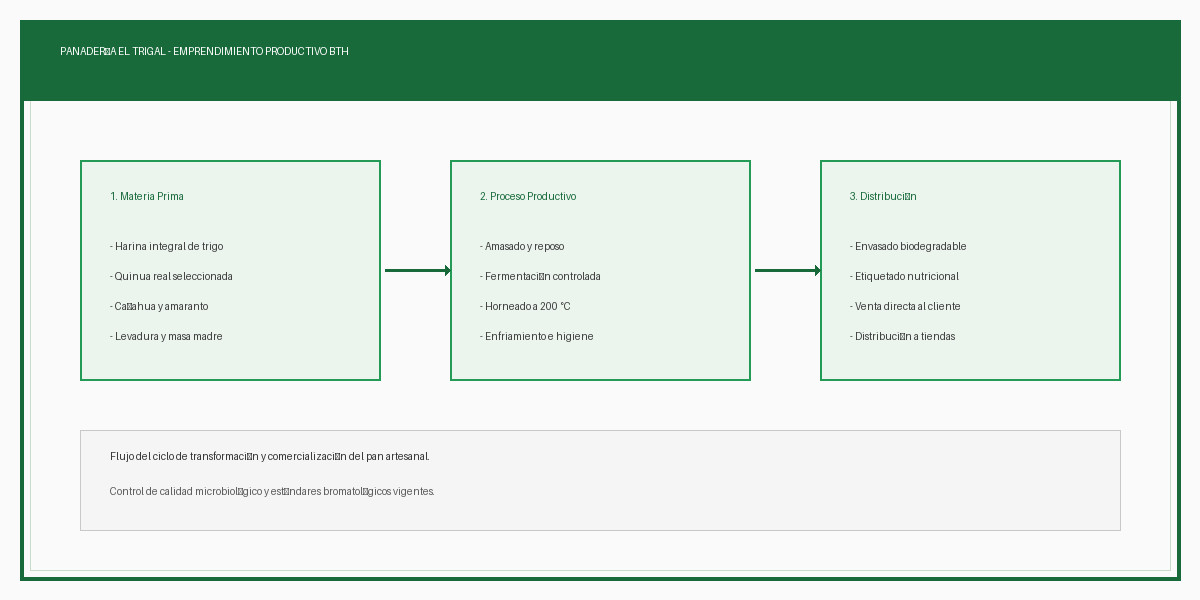
\includegraphics[width=0.85\textwidth]{ejemplo_figura.png}
    \notafigura{Elaboración propia con base en el diseño de operaciones de la microempresa.}
\end{figure}

% ------------------------------------------------------------
% OPCIÓN 2: Macro Semántica Simplificada (\figuraapa)
% ------------------------------------------------------------
% Sintaxis: \figuraapa[opciones_ancho]{archivo}{Título}{etiqueta}{Nota}
%
% \figuraapa[width=0.85\textwidth]{ejemplo_figura.png}%
%   {Diagrama de flujo del ciclo productivo.}%
%   {fig:flujo_simplificado}%
%   {Elaboración propia.}

% ------------------------------------------------------------
% OPCIÓN 3: Subfiguras Comparativas (a y b) con subcaption
% ------------------------------------------------------------
% \begin{figure}[htbp]
%     \caption{Prototipos del producto en etapa preliminar y presentación final.}
%     \label{fig:prototipos_comparativos}
%     \centering
%     \begin{subfigure}[b]{0.45\textwidth}
%         \centering
%         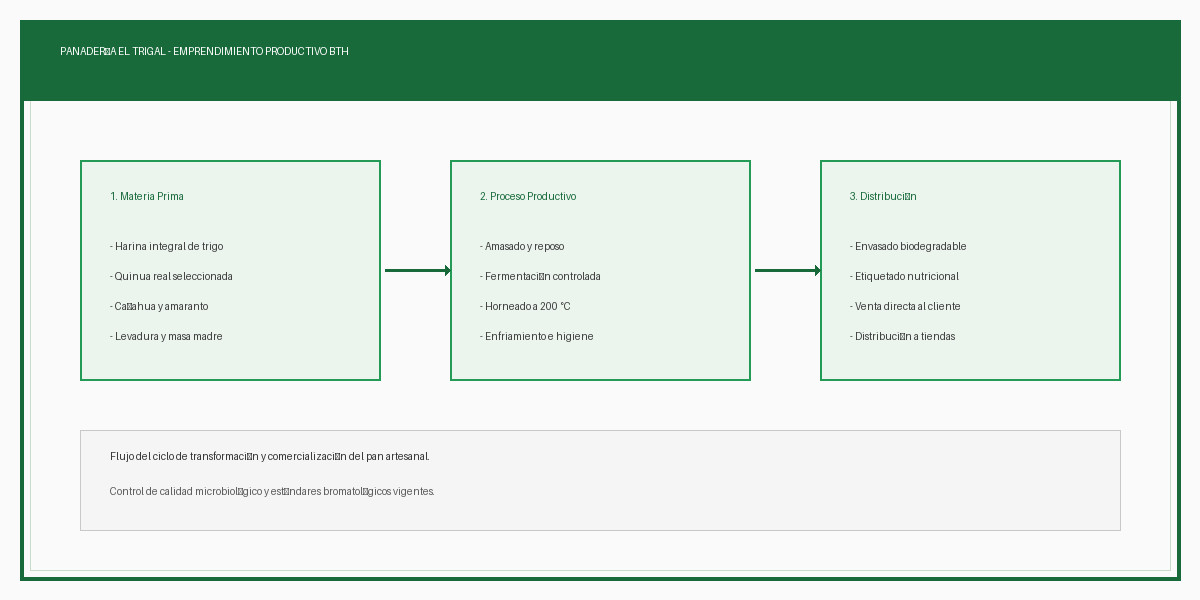
\includegraphics[width=\textwidth]{ejemplo_figura.png}
%         \caption{Prototipo inicial.}
%         \label{subfig:prototipo_inicial}
%     \end{subfigure}
%     \hfill
%     \begin{subfigure}[b]{0.45\textwidth}
%         \centering
%         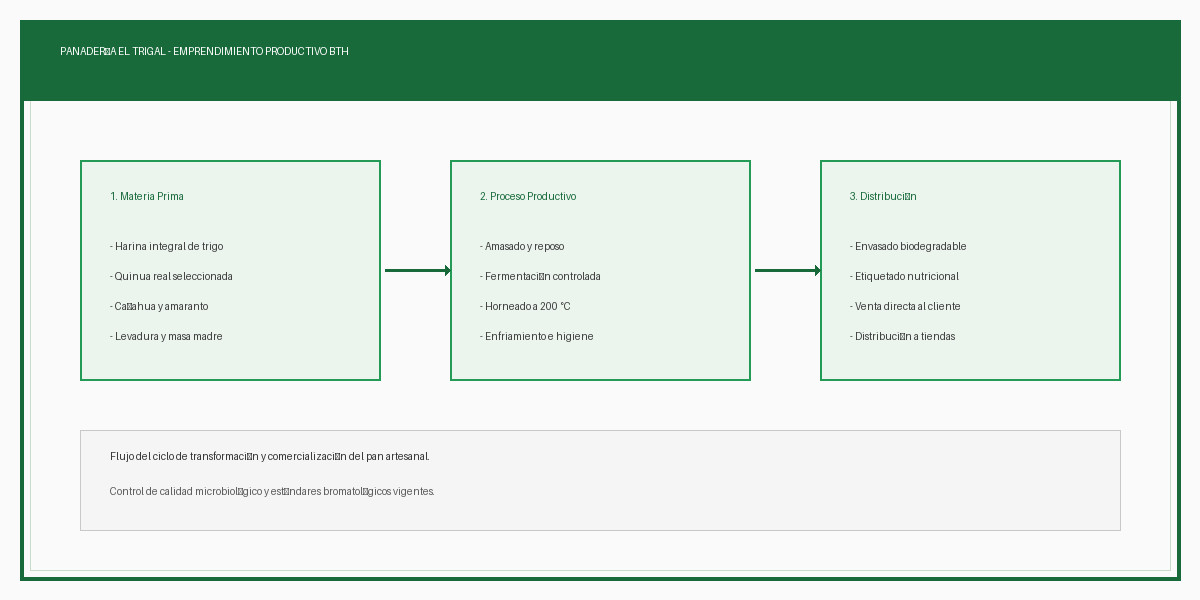
\includegraphics[width=\textwidth]{ejemplo_figura.png}
%         \caption{Empaque final comercial.}
%         \label{subfig:empaque_final}
%     \end{subfigure}
%     \notafigura{Registros fotográficos obtenidos durante las pruebas piloto de laboratorio.}
% \end{figure}

% ------------------------------------------------------------
% OPCIÓN 4: Gráfico o Diagrama Vectorial Nativo (TikZ / Código)
% ------------------------------------------------------------
% \begin{figure}[htbp]
%     \caption{Estructura conceptual del modelo de negocio.}
%     \label{fig:diagrama_conceptual}
%     \centering
%     \begin{tikzpicture}
%         \node[draw=primary, fill=lightgray, rounded corners, inner sep=8pt] (a) {Propuesta de Valor};
%         \node[draw=secondary, fill=lightgray, rounded corners, inner sep=8pt, right=2cm of a] (b) {Segmento de Clientes};
%         \draw[->, thick, primary] (a) -- node[above]{\small Entrega} (b);
%     \end{tikzpicture}
%     \notagrafico{Elaboración propia con base en el marco metodológico del proyecto.}
% \end{figure}

